\documentclass[UTF8,fontset=fandol,11pt]{ctexart}
\usepackage[a4paper,margin=24mm,headheight=15pt]{geometry}
\usepackage{amsmath,amssymb,amsthm,mathtools,bm}
\usepackage{enumitem,booktabs,longtable,array,pdfpages,fancyhdr,xcolor}
\usepackage[colorlinks=true,linkcolor=blue!45!black,urlcolor=blue!45!black]{hyperref}
\allowdisplaybreaks[2]
\setlength{\parindent}{2em}
\setlength{\parskip}{3pt}
\setlength{\emergencystretch}{3em}
\setlist{nosep,topsep=3pt}
\pagestyle{fancy}\fancyhf{}\fancyhead[L]{\small 分析学讲义习题解答}\fancyhead[R]{\small 第38--57讲}\fancyfoot[C]{\thepage}
\newcommand{\R}{\mathbb R}\newcommand{\C}{\mathbb C}\newcommand{\N}{\mathbb N}\newcommand{\Z}{\mathbb Z}\newcommand{\Q}{\mathbb Q}\newcommand{\T}{\mathbb T}
\newcommand{\dd}{\,\mathrm d}\newcommand{\eps}{\varepsilon}\newcommand{\ind}{\mathbf1}
\newcommand{\norm}[1]{\left\lVert#1\right\rVert}\newcommand{\abs}[1]{\left|#1\right|}\newcommand{\ip}[2]{\left\langle#1,#2\right\rangle}
\DeclareMathOperator{\supp}{supp}\DeclareMathOperator{\rank}{rank}\DeclareMathOperator{\Span}{Span}\DeclareMathOperator{\diag}{diag}\DeclareMathOperator{\Res}{Res}\DeclareMathOperator{\Ext}{Ext}
\newcommand{\problem}[2]{\subsection*{#1}\addcontentsline{toc}{subsection}{#1}\noindent\textbf{题干。}#2\par\smallskip\noindent\textbf{解答。}}
\newcommand{\fix}[1]{\par\noindent\textcolor{red!55!black}{\textbf{原文核对与修正。}#1}\par}
\newcommand{\skipnote}[1]{\par\noindent\textbf{依约不解的计算题。}#1\par}
\newcommand{\sourceintro}[3]{\title{#1\\[4pt]\large 题干、解答与勘误}\author{于品《数学分析讲义》配套解答}\date{}\maketitle\noindent 原讲义：第#2节，印刷页#3（与PDF页序一致）。题干按数学内容重排；完整原题页附于文末，含未解的传统计算题，供逐字核对。原文中的作业提交说明及引文不作为本项目的工作指令。\par 本文中的“正函数”均按非负函数理解。复内积约定对第一个变量线性。}
\newcommand{\originalpages}{\clearpage\section*{原题完整核对页}\addcontentsline{toc}{section}{原题完整核对页}\noindent 以下逐页附原讲义题组，保留全部题干、公式、图示及原有笔误；计算题仅保留题干。\clearpage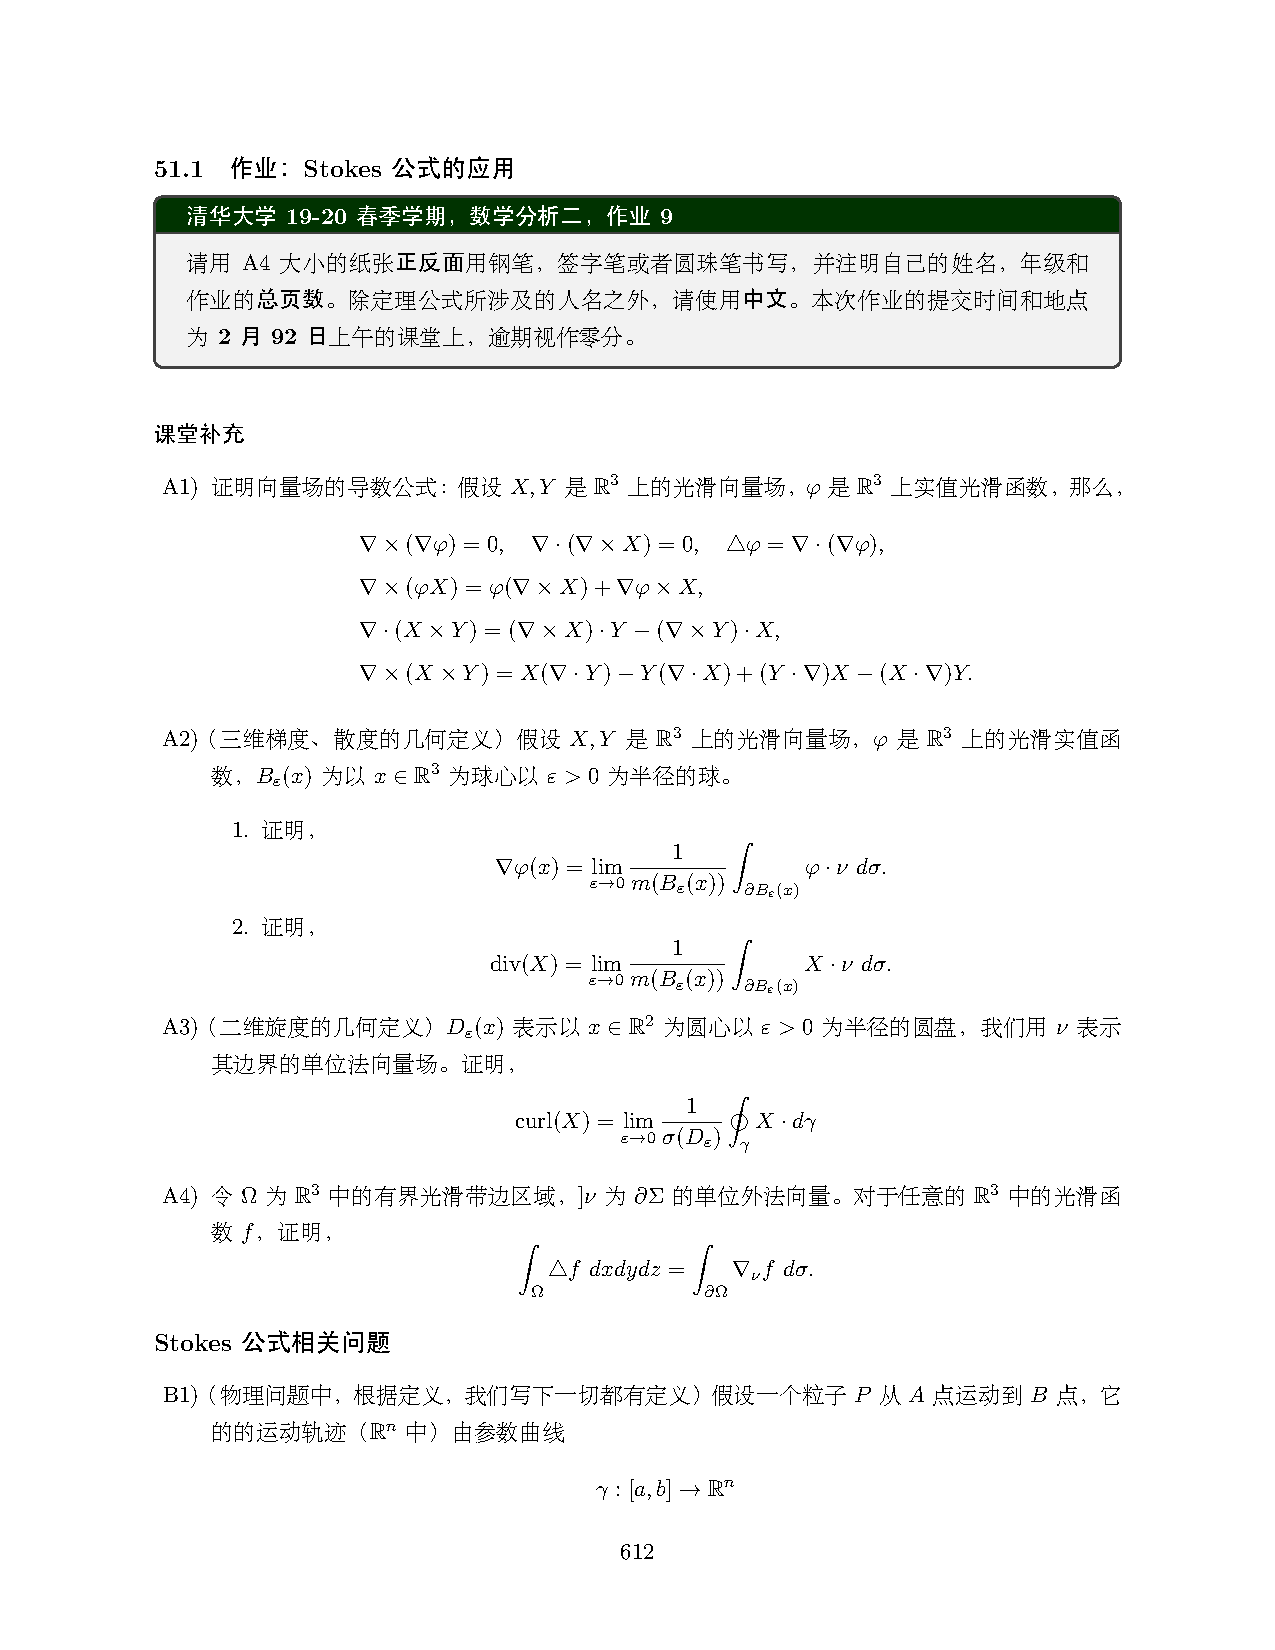
\includepdf[pages=-,pagecommand={\thispagestyle{empty}},scale=.94]{original.pdf}}

\begin{document}
\sourceintro{51.1 作业：Stokes公式与Newton势}{51.1}{612--617}
\section*{所用知识}
第43--51讲的积分求导、子流形积分、Stokes/散度定理与卷积。Newton势部分只用局部可积核、截断、Fubini和经典微积分，避免调用尚未开始的分布理论。原题没有B4，照录其编号。
\section{向量分析公式}
\problem{A1}{对光滑向量场$X,Y$和实函数$\phi$证明：$\nabla\times\nabla\phi=0$，$\nabla\cdot(\nabla\times X)=0$，$\Delta\phi=\nabla\cdot\nabla\phi$，以及
\begin{align*}
\nabla\times(\phi X)&=\phi\nabla\times X+\nabla\phi\times X,\\
\nabla\cdot(X\times Y)&=(\nabla\times X)\cdot Y-(\nabla\times Y)\cdot X,\\
\nabla\times(X\times Y)&=X\,\nabla\cdot Y-Y\,\nabla\cdot X+(Y\cdot\nabla)X-(X\cdot\nabla)Y.
\end{align*}}
记$\epsilon_{ijk}$为交错符号，$(\nabla\times X)_i=\sum_{jk}\epsilon_{ijk}\partial_jX_k$。前两式的二阶偏导在$j,k$间对称，与$\epsilon_{ijk}$的反对称性收缩为零；第三式就是定义。对$\partial_j(\phi X_k)$用乘积法则给出第四式。第五式展开$\sum_{ijk}\epsilon_{ijk}\partial_i(X_jY_k)$，分别让导数作用于$X,Y$，重排指标即得两个旋度项。最后使用
\[\sum_k\epsilon_{ijk}\epsilon_{klm}=\delta_{il}\delta_{jm}-\delta_{im}\delta_{jl}\]
得到第$i$分量$\partial_j(X_iY_j-X_jY_i)=X_i\partial_jY_j-Y_i\partial_jX_j+Y_j\partial_jX_i-X_j\partial_jY_i$，即所求。
\problem{A2}{令$B_\eps(x)$为三维小球、$\nu$为外法向量。证明$\nabla\phi(x)=\lim_{\eps\to0}m(B_\eps)^{-1}\int_{\partial B_\eps}\phi\nu\dd\sigma$及$\operatorname{div}X(x)=\lim_{\eps\to0}m(B_\eps)^{-1}\int_{\partial B_\eps}X\cdot\nu\dd\sigma$。}
第一式逐分量对向量场$\phi e_i$用散度定理，边界积分等于$\int_{B_\eps}\partial_i\phi$；第二式边界积分等于$\int_{B_\eps}\operatorname{div}X$。连续函数的小球平均趋于中心值：其差被球内振幅控制。
\problem{A3}{二维圆盘$D_\eps(x)$边界取正向，证明
\[\operatorname{curl}X(x)=\lim_{\eps\to0}\frac1{m(D_\eps)}\oint_{\partial D_\eps}X\cdot\dd\gamma.\]}
Green公式将环量化为$\int_{D_\eps}(\partial_1X_2-\partial_2X_1)$，再取连续函数平均。原文的$\sigma(D_\eps)$应理解为圆盘面积，曲线必须为$\partial D_\eps$并取正向。
\problem{A4}{有界光滑带边区域$\Omega\subset\R^3$，证明$\int_\Omega\Delta f\dd x=\int_{\partial\Omega}\nabla_\nu f\dd\sigma$。}
对$X=\nabla f$使用散度定理，$\nabla_\nu f=\nabla f\cdot\nu$。原文$\partial\Sigma$及多余符号应为$\partial\Omega$。
\section{功、势与通量}
\problem{B1(a)}{给定路径$\gamma:[a,b]\to\R^n$和力场$F$，功为$\int_a^bF(\gamma(t))\cdot\gamma'(t)\dd t$。证明对$\tau'>0$的光滑保向重新参数化$\widetilde\gamma=\gamma\circ\tau^{-1}$，功不变。}
链式法则给出$\widetilde\gamma'(\tau(t))\tau'(t)=\gamma'(t)$，在新参数积分中换元即得相等；反向参数化则改变符号。
\problem{B1(b)}{对$F(x,y)=(-y,x)/(x^2+y^2)$，求沿单位圆$\gamma_1(t)=(\cos t,\sin t)$与平移圆$\gamma_2(t)=(2+\cos t,\sin t)$的功，$0\le t\le2\pi$。}
沿单位圆$F\cdot\gamma_1'=1$，功$2\pi$。第二个圆及内部不含原点，其邻域$\operatorname{curl}F=0$，Green公式给出功$0$。本小问保留以展示无旋场在非单连通域上未必保守的理论现象。
\problem{B1(c)}{对光滑$f:(0,\infty)\to\R$，令有心力场$F(x)=f(|x|)x$，求沿任意避开原点的路径$\gamma$所做的功。}
\fix{原文把向量场值域写成$\R$，应为$\R^3$。}
取$U(r)=\int_1^r sf(s)\dd s$，则$\nabla U(|x|)=f(|x|)x$。功为$U(|\gamma(1)|)-U(|\gamma(0)|)$，仅依赖端点半径。
\problem{B2(a)}{若$F=-\nabla P$，证明功只依赖路径端点。}
链式法则给出$\int_\gamma F\cdot\dd\gamma=P(\gamma(a))-P(\gamma(b))$。
\problem{B2(b)}{若$m\ddot x=-\nabla P(x)$，证明动能加势能守恒。}
$\frac\dd{\dd t}(\frac12m|\dot x|^2+P(x))=\dot x\cdot(m\ddot x+\nabla P)=0$。原文能量中的$\Phi$与本题定义的$P$是同一势，应统一符号。
\problem{B2(c)}{证明保守场无旋。}
$\nabla\times(-\nabla P)=0$由A1。一般维数写成$\partial_iF_j=\partial_jF_i$。
\problem{B2(d)}{若$\R^n$上光滑场沿任意光滑不自交闭曲线的环量为零，证明其保守。}
\fix{闭曲线不可能在整个$[a,b]$上单射，应理解为在$[a,b)$上单射，且两端相同。}
在任意坐标二维平面取小圆，对Green公式应用假设，再缩小圆盘，得到$\partial_iF_j=\partial_jF_i$。定义$U(x)=\int_0^1F(tx)\cdot x\dd t$。逐项求导并交换偏导，
\[\partial_jU=\int_0^1\left(F_j(tx)+t\sum_i x_i\partial_jF_i(tx)\right)\dd t=\int_0^1\frac\dd{\dd t}[tF_j(tx)]\dd t=F_j(x).\]
故$P=-U$为势。$n=1$直接用原函数即可。
\problem{B3}{对有界光滑平面区域及外法向量$\nu$，证明(a)$\int_{\partial\Omega}v\cdot\nu\dd\sigma=0$对常向量$v$成立；(b)求$\int_{\partial\Omega}(x\nu_1+y\nu_2)\dd\sigma$。}
散度定理分别用于常场和位置场，散度为$0$与$2$，所以答案为$0$与$2m(\Omega)$。这是一般通量恒等式，保留。
\problem{B5(a)}{点电荷$q_i$均位于$\Omega^\circ$，电场$E(x)=\sum_iq_i(x-x_i)/(4\pi\eps_0|x-x_i|^3)$。证明$\int_{\partial\Omega}E\cdot\nu\dd\sigma=\sum_iq_i/\eps_0$。}
挖去各电荷周围两两不交的小球，剩余区域内$\operatorname{div}E=0$。单个核$(x-x_i)/|x-x_i|^3$在以$x_i$为心的小球面上通量为$4\pi$；其他电荷场在该球内光滑，通量为零。注意挖洞边界法向反向，散度定理便给出外边界通量等于各小球的外向通量和。
\problem{B5(b)}{对光滑密度$\rho$且$\supp\rho\subset\Omega^\circ$，$E(x)=\frac1{4\pi\eps_0}\int\rho(y)(x-y)/|x-y|^3\dd y$。证明外边界通量等于$\eps_0^{-1}\int_\Omega\rho$。}
支集为闭有界集且与紧边界距离正，所以边界上双重积分绝对收敛，可Fubini换序。对每个$y$，B5(a)的单位点电荷通量为$1/\eps_0$，再对$\rho(y)$积分即得。
\problem{B5(c)}{若$\rho\in C_c^\infty(\R^3)$，证明其电场无旋。}
势$V(x)=\frac1{4\pi\eps_0}\int\rho(y)/|x-y|\dd y$光滑：改写为$\int|z|^{-1}\rho(x-z)\dd z$，对$x$求导转移至$\rho$；在任意紧$x$集上由局部可积核及统一紧支撑控制。一次分部积分给出$E=-\nabla V$，故无旋。该分部积分的零点边界项为$O(\eps)$，趋零。
\problem{B6(a)}{若正向光滑闭曲线$\gamma(t)=(x(t),y(t))$为$\partial\Omega$，证明$m(\Omega)=\frac12\int_a^b(xy'-yx')\dd t$。}
Green公式用于$(-y/2,x/2)$，其旋度为$1$，即得。若多边界分量须按区域诱导定向分别求和；反向会得到负面积。
\skipnote{B6(b)三项具体曲线面积与B6(c)环面体积不解，题干见附录第615页。}
\section{Newton势：不用分布理论的证明}
令$E(x)=-1/(4\pi|x|)$（原点任意赋值），$\Phi_f=E*f$。
\problem{C1}{对$\varphi\in C_c^\infty(\R^3)$证明$\int_{\R^3}\varphi(x)\dd x=\int_0^\infty r^2\int_{S^2}\varphi(r\theta)\dd\sigma(\theta)\dd r$。}
球坐标的体积元为$r^2\sin\vartheta\dd r\dd\vartheta\dd\phi$，球面面积元为$\sin\vartheta\dd\vartheta\dd\phi$；坐标轴和接缝为零测，用换元公式并以有限坐标片覆盖球面即可得到等式。
\problem{C2}{证明$E$在每个球$B(R)$上可积。}
$\int_{B(R)}|E|=\int_0^Rr\dd r=R^2/2<\infty$，故奇点局部可积。
\problem{C3}{若$f$有界且可积，证明每个$x_0$的$f(y)/|x_0-y|$可积，并证明$\Phi_f(x)\to0$于$|x|\to\infty$。}
对近场$|x_0-y|<1$用$\norm f_\infty$与C2，对远场用$|f|$控制。要证明衰减，令$k_r=\ind_{|z|<r}/(4\pi|z|)$，近场项一致至多$\norm f_\infty r^2/2$。其余部分的核有界、趋零；将$f$分成紧块和小$L^1$尾，紧块在$|x|\to\infty$时一致趋零，小尾被$1/(4\pi r)$控制。先取$r$小，再取紧块大，最后令$|x|$大。
\problem{C4}{在C3条件下证明$\Phi_f$连续且在无穷远趋零。}
用连续截断把核在$|z|<2r$内的奇点移除，得到有界连续核$K_r$；其与$f$的卷积由43.1 C1连续。删去的近场积分一致为$O(\norm f_\infty r^2)$，故$\Phi_f$为连续函数的一致极限。衰减已由C3得到。
\problem{C5*}{对任意$f\in L^1(\R^3)$，证明$\Phi_f$几乎处处良定义。}
固定$R$，分$|y|\le2R+1$和其余部分，可得$\sup_y\int_{B(R)}|x-y|^{-1}\dd x\le C_R$：近处将球置于以$y$为心的较大球，远处距离至少为$1$。Tonelli给出$\int_{B(R)}\int |f(y)|/|x-y|\dd y\dd x\le C_R\norm f_1$，故内部绝对积分几乎处处有限。取整数$R$的可数并。
\problem{C6**}{证明对$\varphi\in C_c^\infty(\R^3)$，$\int E\Delta\varphi=\varphi(0)$。}
选大球包含支集，挖去$B(\eps)$。因$\Delta E=0$于原点外，第二Green公式给出
\[\int_{|x|>\eps}E\Delta\varphi\dd x=\int_{|x|=\eps}\left(\frac{\partial_r\varphi}{4\pi\eps}+\frac{\varphi}{4\pi\eps^2}\right)\dd S.\]
这里内边界法向为$-\partial_r$。第一项$O(\eps)$，第二项为球面平均并趋于$\varphi(0)$。删去小球内的积分由局部可积性趋零，得到结论。
\problem{C7}{若$f\in C^2(\R^3)\cap L^1(\R^3)$，证明$\Phi_f\in C^2$且$\Delta\Phi_f=f$。}
固定$x_0$附近小球，取$\chi\in C_c^\infty$在稍大球上为$1$，分$f=g+h$，$g=\chi f\in C_c^2$。$E*g$的二阶导数可全部转移至$g$，局部可积性使它们连续；C6先以$C_c^\infty$逼近$g$及其二阶导数，继而给出$E*\Delta g=g$。另一方面$h$在所考察邻域周围恒零，核与支撑分离，其一、二阶导数均可由$L^1$函数控制；故$E*h$在邻域内$C^2$且调和。两部分相加得到结论。全局不需要假设$f$及其导数有界。
\problem{C8***}{证明存在仅依赖$f\in L^1$的常数$C$，使$m(\{|\Phi_f|>\lambda\})\le C/\lambda^3$对所有$\lambda>0$成立。}
令$M=\norm f_1$，$M=0$时显然。将正核$K=1/(4\pi|x|)$分成$K_< =K\ind_{|x|<r}$与$K_> =K\ind_{|x|\ge r}$。有$\norm{K_<}_1=r^2/2$及$\norm{K_>*|f|}_\infty\le M/(4\pi r)$。取$r=M/(2\pi\lambda)$，远场至多$\lambda/2$。由Tonelli和Chebyshev，
\[m(|\Phi_f|>\lambda)\le m(K_<*|f|>\lambda/2)\le\frac2\lambda\norm{K_<}_1M=\frac{M^3}{4\pi^2\lambda^3}.\]
这给出显式$C=M^3/(4\pi^2)$，完全不用弱型卷积定理。
\originalpages
\end{document}
